
\subsection{Dataflow}
In this section I will describe the dataflow shown in Figure \ref{fig:optimizedfilter}.  The figure outlines the top level components that are described later in section \ref{sec:vhdldesign}.  

We designed the filter to have 7 16-bit registers.  Each of the 7 registers' data is connected to the next register.  At each clock pulse, the registers' data is shifted to the next register. The input is placed at $D0$ and the value stored in $D6$ is not saved.

For $D0$ through $D2$, the registers' output is also connected to an adder.  Because the filter is symmetric, we are able to add two register values together before multiplying by the constants $C0$ through $C2$.  After the addition, the values are multiplied by the constants specified in Table \ref{tab:coefficients}.  The products are then summed using three ripple-carry adders.


\subsection{VHDL Design}
\label{sec:vhdldesign}
We decided to design our filter using as much HDL as possible.  Therefore, every component is written in VHDL, and are synthesized for the final design. The VHDL is separated into components listed below.  These components are then synthesized using the \texttt{rc} and Encounter cadence synthesizer.  

Separate components:
\begin{itemize}
\item \verb=SHIFT_REG=: Shift Register (Appendix \ref{lst:shiftreg.vhd})
	\begin{itemize}
		\item \verb=D_FF=: D-Flip Flop (Appendix \ref{lst:dff.vhd})
	\end{itemize}
\item \verb=CONV_MULT=: Convolution (Appendix \ref{lst:convmult.vhd})
\item \verb=SUM=: Summation (Appendix \ref{lst:sum.vhd})
	\begin{itemize}
		\item \verb=ADD16=: 16-Bit Adder (Appendix \ref{lst:add16.vhd})
		\begin{itemize}
			\item \verb=FULL_ADDER=: Full Adder (Appendix \ref{lst:fulladder.vhd})
		\end{itemize}
	\end{itemize}
\end{itemize}

The source of the VHDL components are included in the appendix.  

During early synthesis, we found that the standard libraries did not have a flip-flop available.  We needed a flip-flop in order to create our registers.  Therefore, we created a D Flip Flop using the structural specification.


\subsection{Functional Verification}
To verify the correctness of the VHDL design files, we have written a C++ program that generates test cases. This program first generates test input with random noise. Then it computes the output using the equivalent filter algorithm in Q15 format. The result is stored in a text file (Appendix \ref{lst:testcase.txt}) which can be read by a VHDL testbench \texttt{filter\_tb.vhd} (Appendix \ref{lst:filter_tb.vhd}).

\begin{figure}[ht]
	\centering
	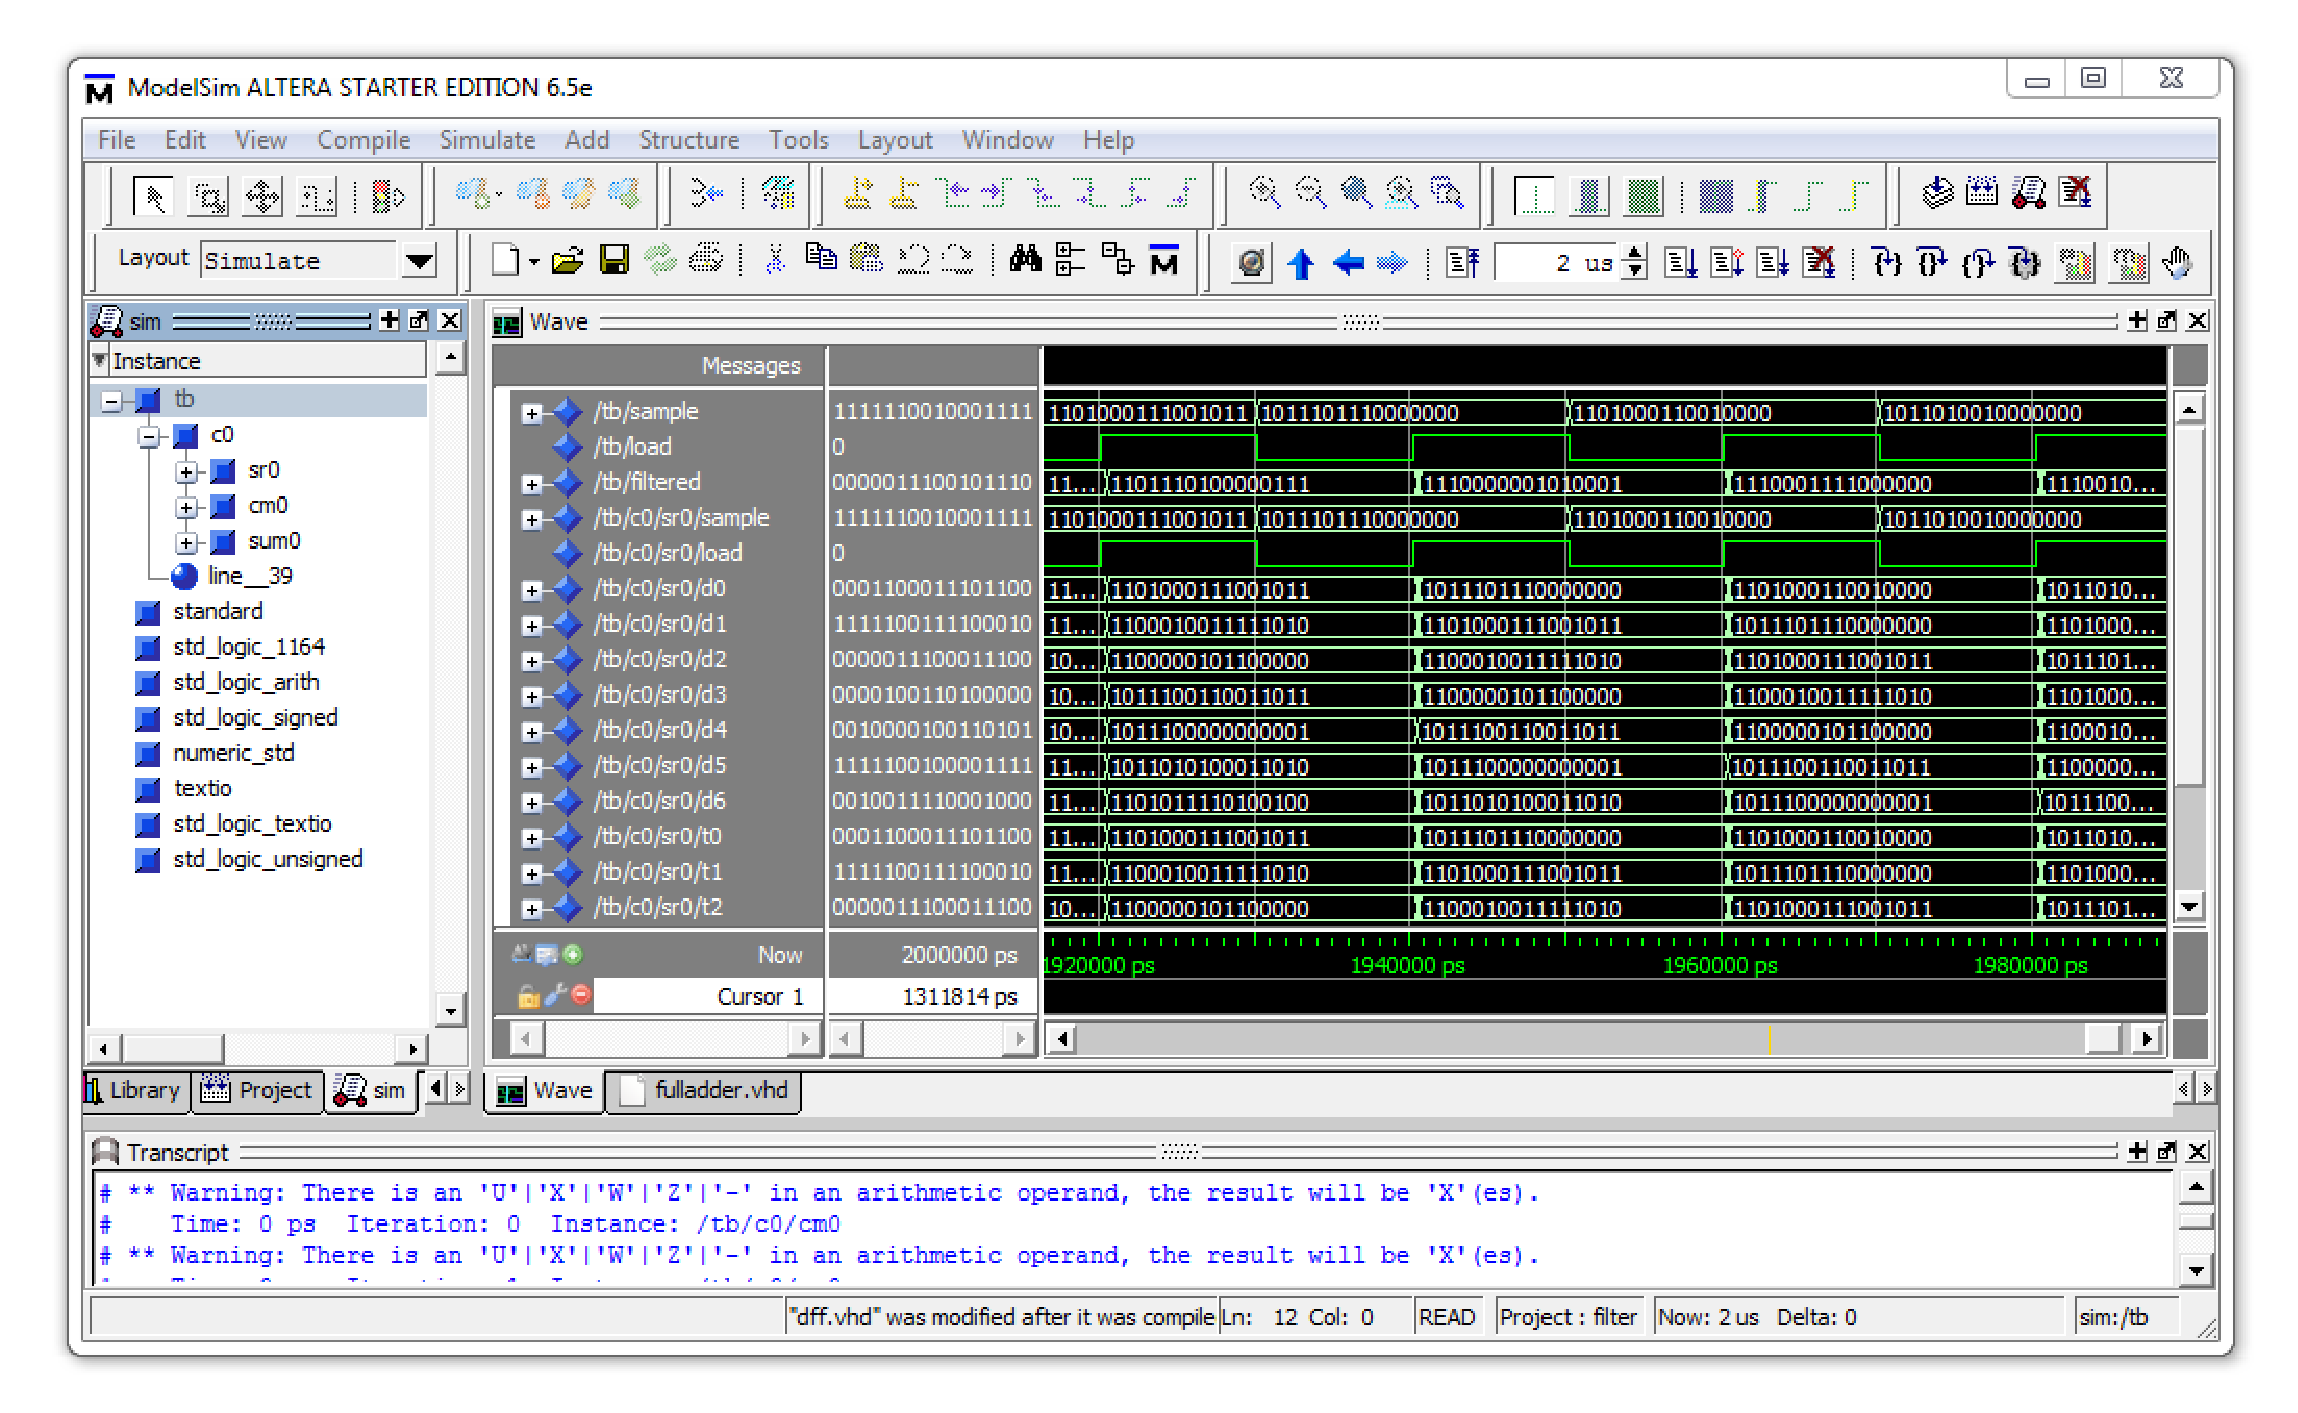
\includegraphics[width=6.5in]{images/modelsim}
	\caption{ModelSim from Mentor Graphics was used for VHDL simulation.}
	\label{fig:q7}
\end{figure}

For VHDL simulation, we used ModelSim from Mentor Graphics. This tools loads and compiles all VHDL files including the test bench, then shows the waveform and output to the window. Our testbench file follows the VHDL standard and prints the results into a text file, so it should work on other environments other than ModelSim.

We verified that the every bit of the C++ program output and VHDL testbench output matched, therefore the VHDL should be correct with high probability.


\subsection{Synthesis}

Synthesis was done using rc cadence synthesizer and the Encounter tool.  For the encounter tool, we followed the instructions listed in lab 3.  The Encounter routing and placement on the \verb=CONV_MULT= component took 45 minutes to complete while the FullAdder was near instant.  See Figure \ref{fig:convmult} for the synthesized convolution hardware.

\begin{figure}[htbp]
\centering
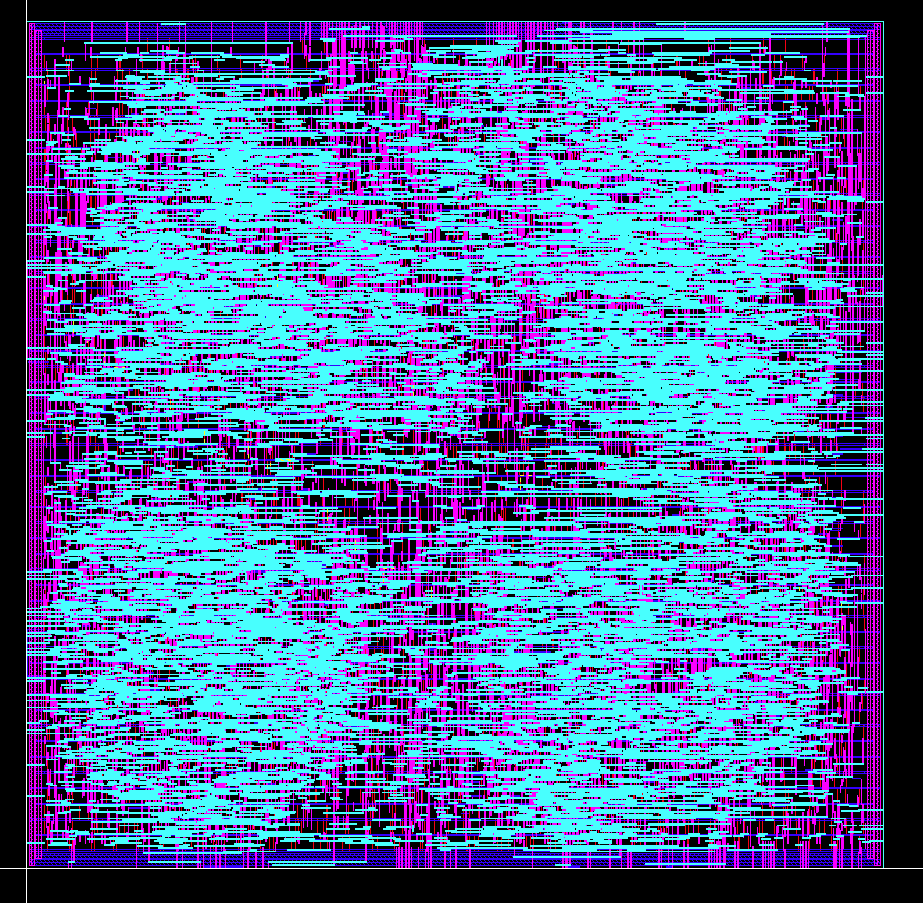
\includegraphics[width=6.5in]{images/CONV_MULT}
\caption{Convolution hardware after synthesis.}
\label{fig:convmult}
\end{figure}


\subsection{Final Layout \& Routing}
Since each component was designed in a separate VHDL file, they had to be connected at a high level.  See Figure \ref{fig:filterschematic} for the schematic of the connected high level components.  This logical layout closely resembles the layout shown in Figure \ref{fig:optimizedfilter}.

% 2500x2500 
After creating the schematic, we used the Cadence router to route between the top level components.  The chip size needed to be increased to 2500x2500 microns in order to accommodate the components.  The convolution chip alone is 1500x1500 microns.  The routing completes in about an hour with no un-routable endpoints.  See Figure \ref{fig:filterrouted} for the routed final layout.


\begin{figure}[htbp]
\centering
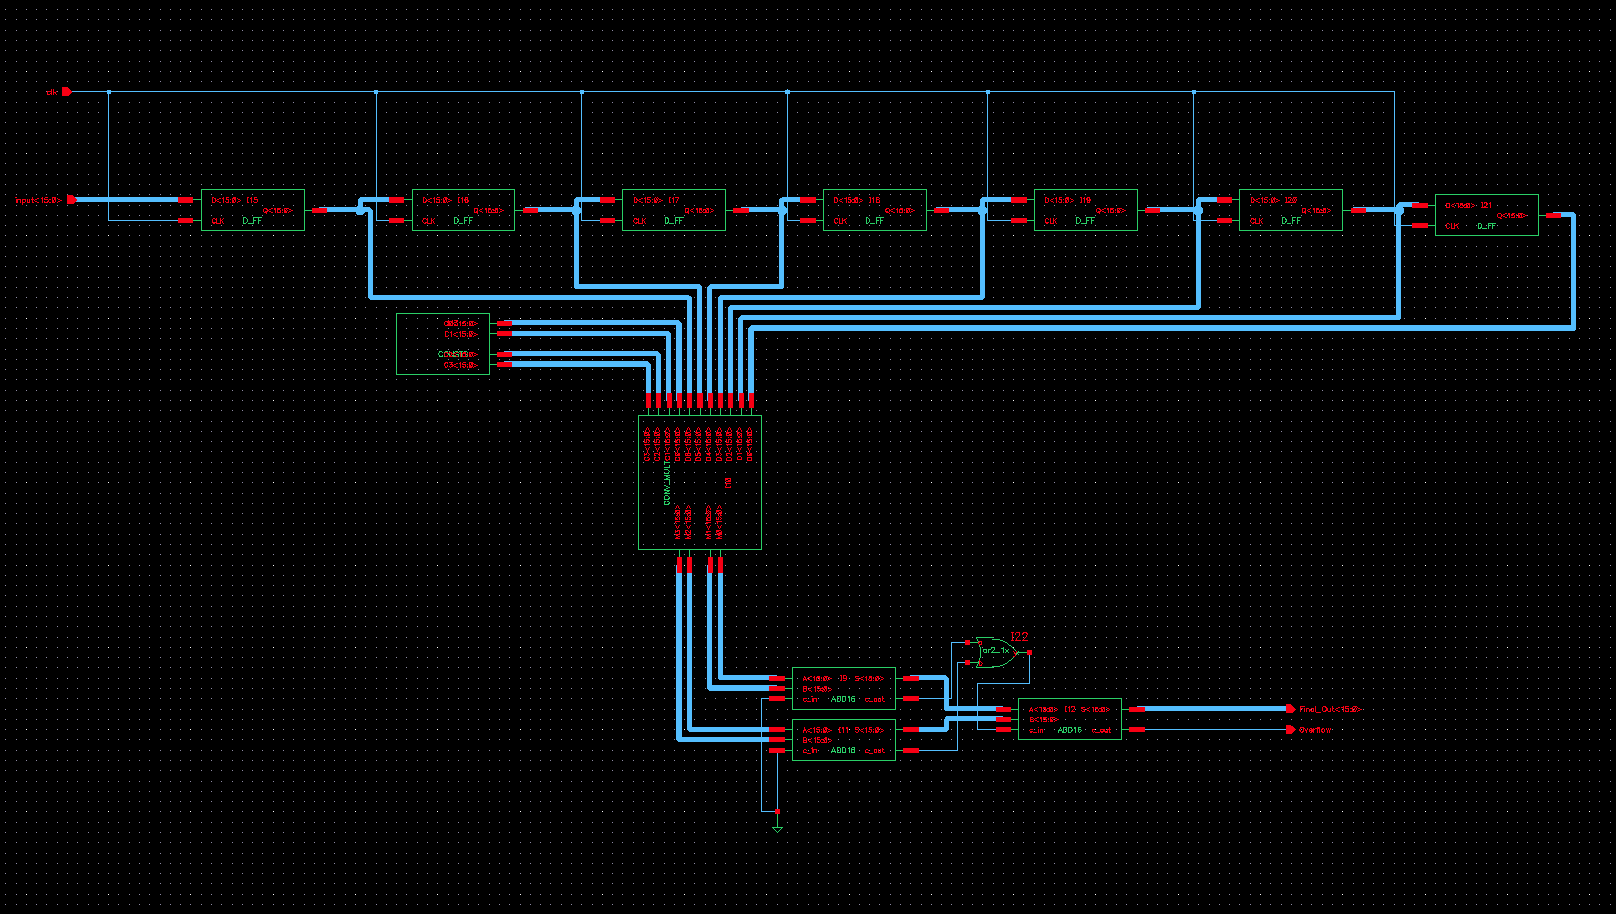
\includegraphics[angle=90,height=8in]{images/Filter-Schematic}
\caption{Filter Schematic.}
\label{fig:filterschematic}
\end{figure}


\begin{figure}[htbp]
\centering
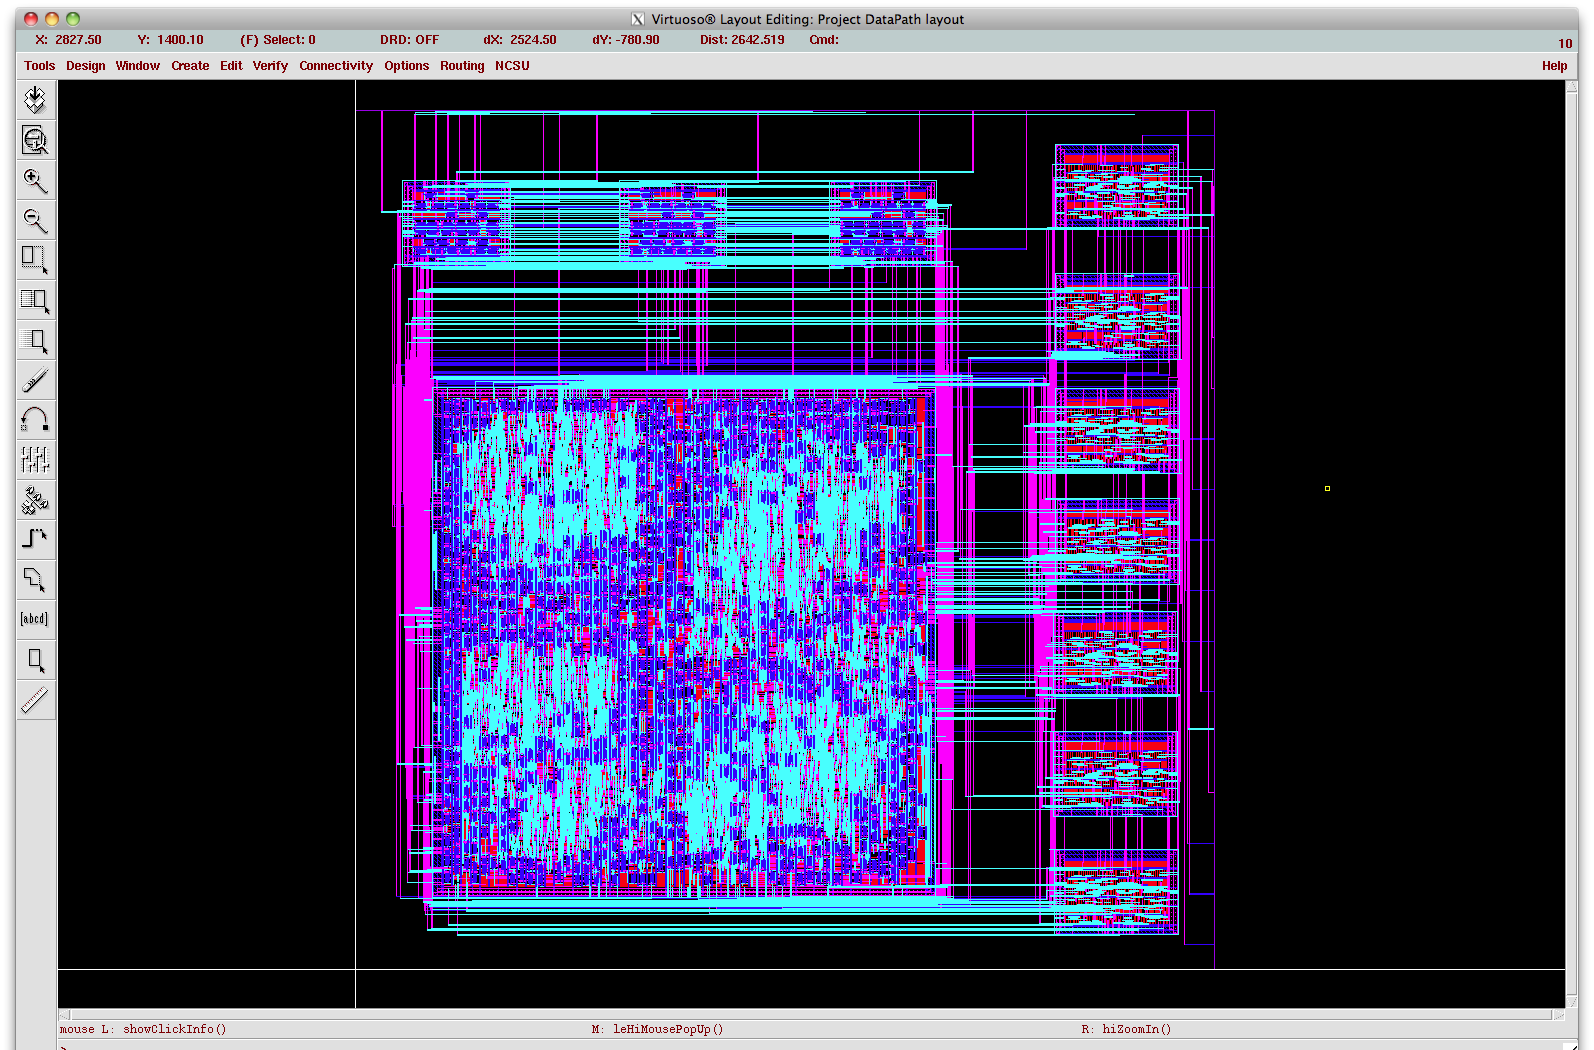
\includegraphics[angle=90,height=8in]{images/FinalRouted}
\caption{Filter Routed.}
\label{fig:filterrouted}
\end{figure}





